\documentclass[a4paper, 11pt, titlepage]{jsarticle}
\usepackage[dvipdfmx]{hyperref,graphicx}
\usepackage{listings}
\usepackage{amsmath}
\usepackage{url}
\usepackage{here}

\title{知能情報実験III(データマイニング班)\\Twitter上のテキスト文を対象とした「コロナで何が困っているのか」を見つける}
\author{グループの学籍番号 205759A, 205720E, 205763J, 195719J}
\date{提出日:2022年6月9日}
\begin{document}
\maketitle
\tableofcontents
\clearpage

\section{はじめに}
\subsection{概要}
本実験では、グループでテーマを決めて、半年間でデータ解析に取り組むグループワークである。グループワークを通して、機械学習や実験再現のためのドキュメント作成等を目指す。

\subsection{テーマ:Twitter上のテキスト文を対象とした「コロナで何が困っているのか」を見つけるとは}
本グループではTwitter上のテキスト文を対象として「コロナで困っていること」を見つけることを対象問題として設定した。SNSを使ってコロナで発生している問題を可視化し、件数が多い項目を整理することで、その後の改善策を見出して今後に応用できる。それによって現在発生している問題に対処しつつ今後同様の問題が発生する際により効果的な対策ができるようになることが期待できる。

\section{実験方法}
\subsection{実験目的}
コロナで何が困っているのかがわかることでその後の改善策を見出すことができ、今後に応用するために、Twitter上のテキスト文を用いて解析する。


%Twitter上のテキスト文を対象として「コロナで何が困っているのか」という事柄を視覚的にわかるようした。具体的な内容として、まず、Twitter上のテキスト文のなかから「コロナ」という単語が含まれた文章を抽出し、ネガティブかポジティブかの判定を行った。次に、その結果の中からネガティブな文章を取り出し、クラスタリングを行った。最後に、クラスタリングされた事柄の中で発言している人数が多い順に順位付けを行うことで優先的に対処しなければならない事柄を視覚的にわかるようにした。

\subsection{データセット構築}
Twitterscraping.pyを実行することで、Pythonのsnscrapeライブラリ・モジュールを使用して、Twitter上のテキスト文のなかから「コロナ」という単語が含まれた文章を抽出し、それらをデータセットとしてsample.csvに出力した\cite{snscrape}。次に、extract\_content.pyを実行してsample.csvを読み込み、contentカラムだけを取り出すことで、tweetの文章だけをcontent.csvに出力した。negaposi.pyを実行することで、このcsvファイルと、日本語評価極性辞書を利用したPython用Sentiment Analysisライブラリosetiを使ってネガティブとポジティブに分けた\cite{oseti}。そして、ネガティブに判定されたtweetだけを抽出し、nega.csvに出力した。

\subsection{モデル選定}
実験目的に沿って、教師なし学習で文書のクラスタリングを行うためLDA(トピックモデル)を使用した。また、トピックモデルはpyLDAvisを用いてインタラクティブに可視化できる部分もLDAを選んだ理由である。 

\subsection{パラメータ調整}
クラスター数(カテゴリ数)の最適数を見つけるため、クラスター数3〜50の結果をメンバーで確認し、トピック名をつけやすいクラスター数を探した。また、その他のパラメータは参考にしたサイトの値をそのまま使用した\cite{LDA}。

\section{実験結果}
pyLDAvisを使用してトピックモデリングの内容をhtmlに出力した結果は以下の通りである。\href{https://ie.u-ryukyu.ac.jp/~e205759/pyldavis_output.html}{(リンク)}\\
 まず出力されたIntertopic Distance Mapの分布の見方から説明する。\\
\begin{figure}[H]
  \centering 
  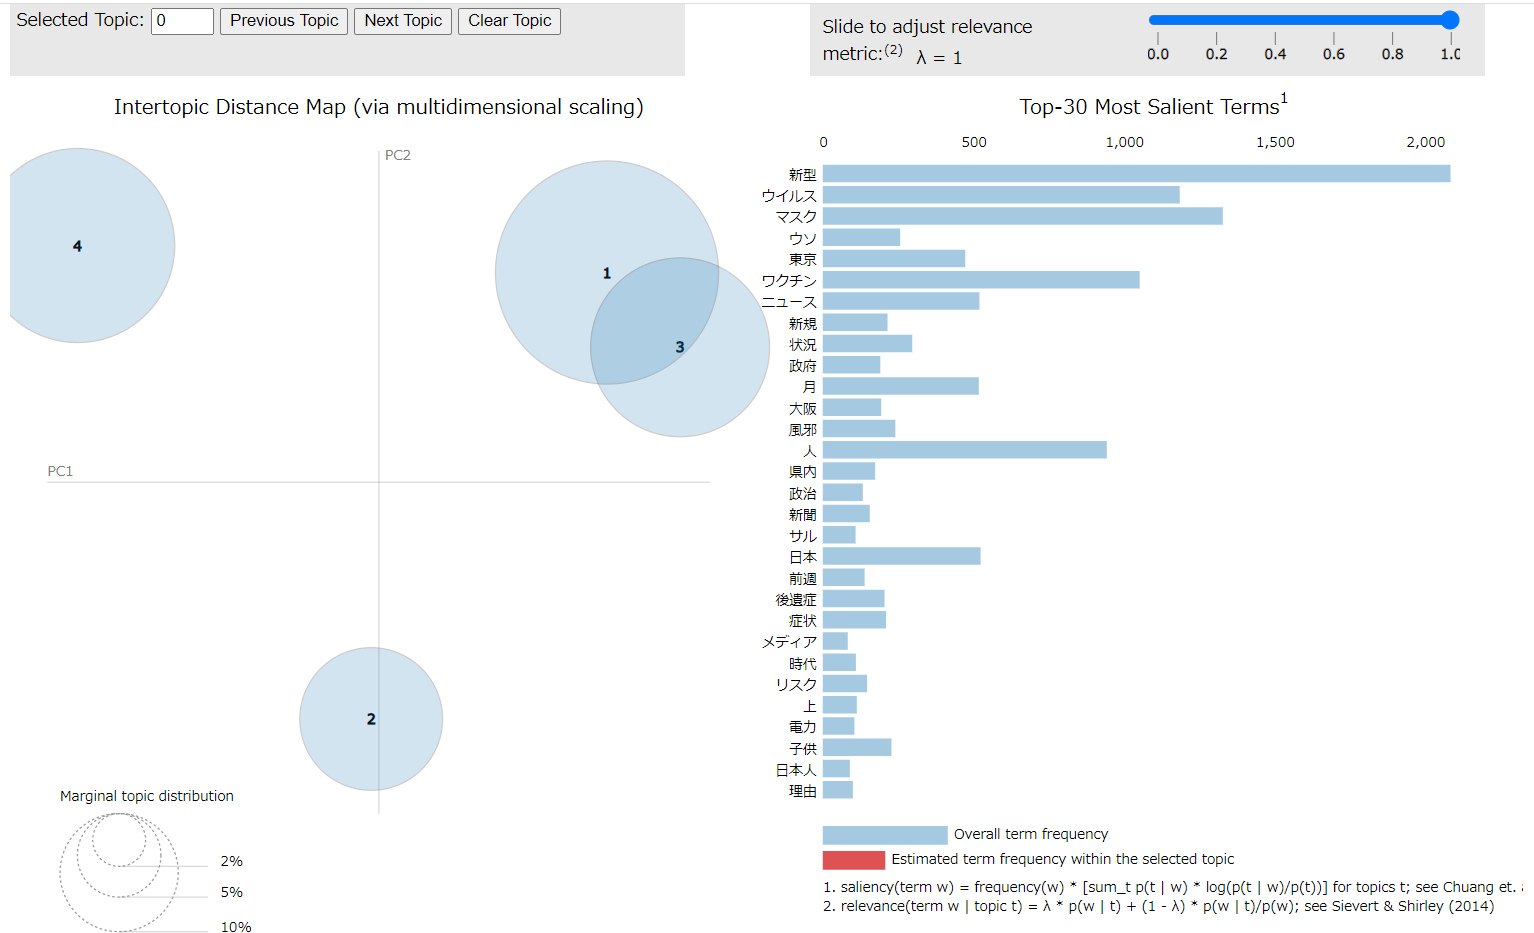
\includegraphics[scale=0.25]{picture1.png}
  \caption{トピックモデリングの出力結果}
\end{figure}
図1の左側には各トピックを多次元尺度法(MDS)で2次元に落として配置したものが表示され、円の大きさは全体の単語に対する、各トピックに所属する単語の割合を表している。また、右側には選択したトピックにおける頻出単語、同トピック内での出現頻度が大きい単語とその頻度が表示される。右上にあるパラメータλを変えると出現頻度、同トピック内での出現頻度の割合の比率を変えて順位を変えられる。右側の単語にマウスを重ねると各トピック内における出現頻度が左側の円の大きさとして表示される。\\
\newpage
図1によるとクラス1と3は似たトピックで、2と4はそれぞれ離れたトピックであることがわかる。また、全てのツイートに含まれている「コロナ」という単語を除くと、図2,3より、1と3のトピックで多く含まれる単語は「ワクチン」、「マスク」、「人」であり、また、「風邪」「症状」や「後遺症」という単語が1のトピックのみに含まれている。\\
\begin{figure}[H]
  \centering
  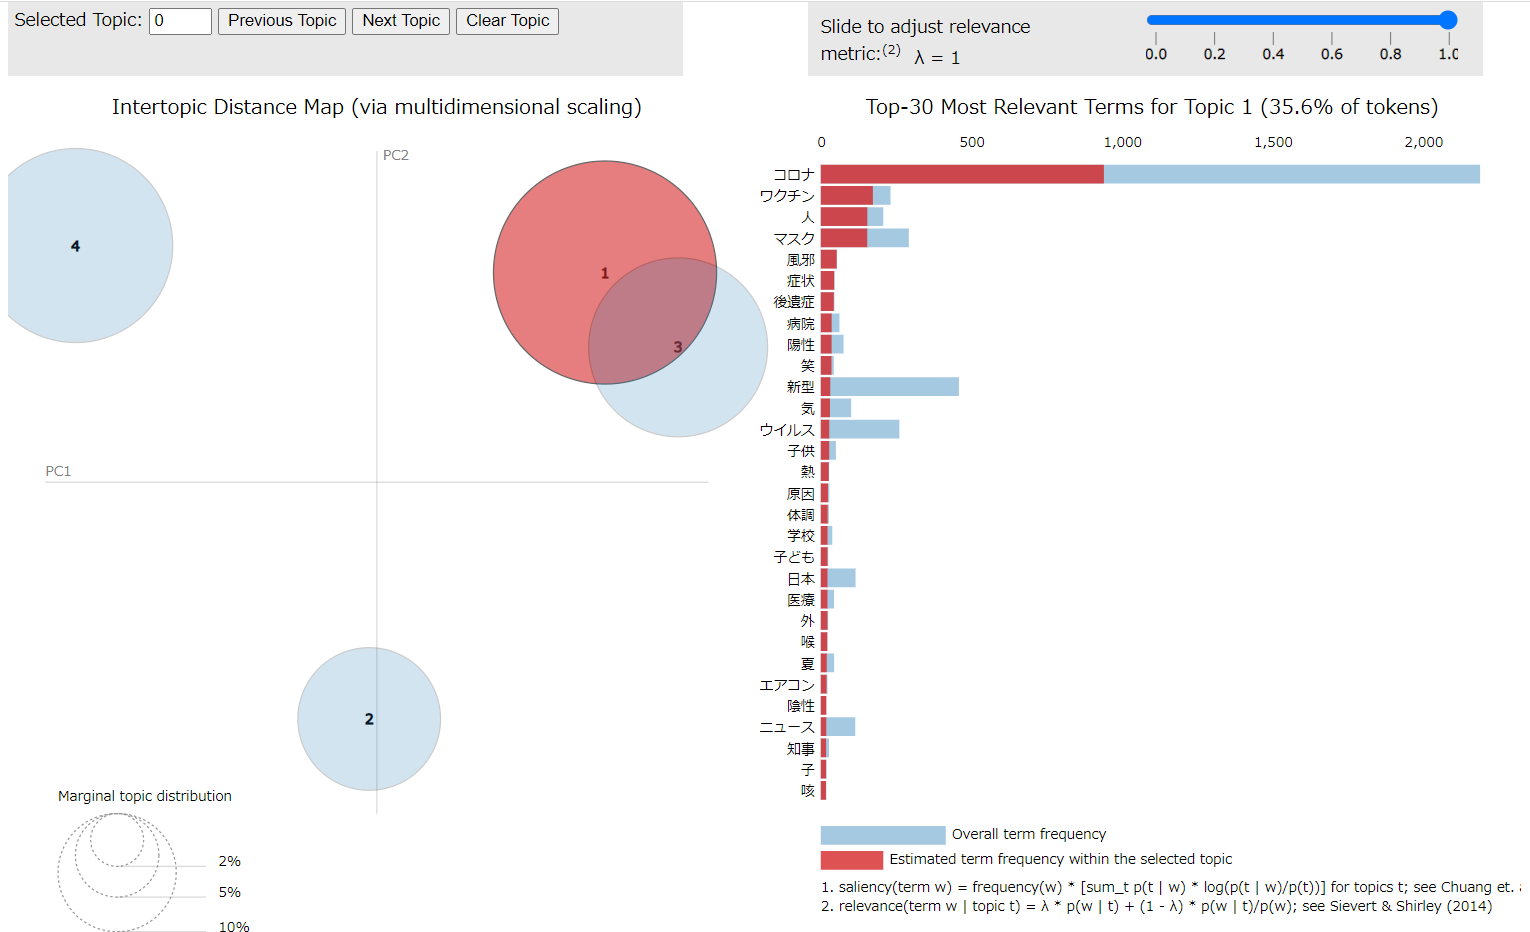
\includegraphics[scale=0.25]{picture2.png}
  \caption{クラス1の単語数}
  \centering
  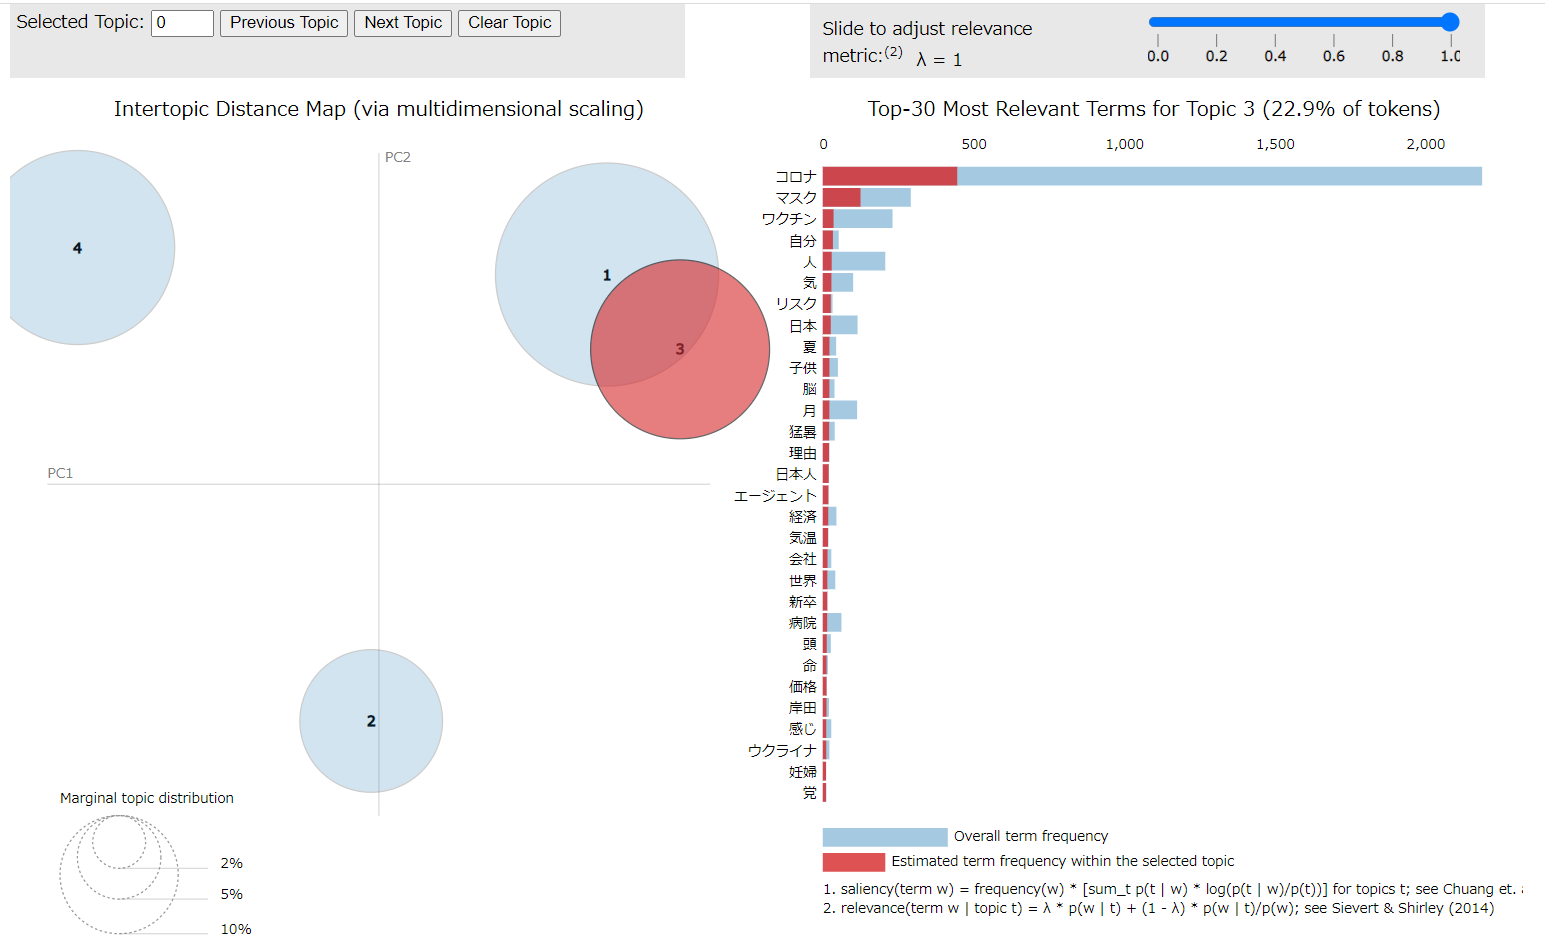
\includegraphics[scale=0.25]{picture3.png}
  \caption{クラス3の単語数}
\end{figure}
\newpage
図4を見ると、2のトピックで多い単語は「新型」「ウソ」「日本」であり、さらに、「政府」や「政治」という単語が多い。\\
\begin{figure}[H]
  \centering
  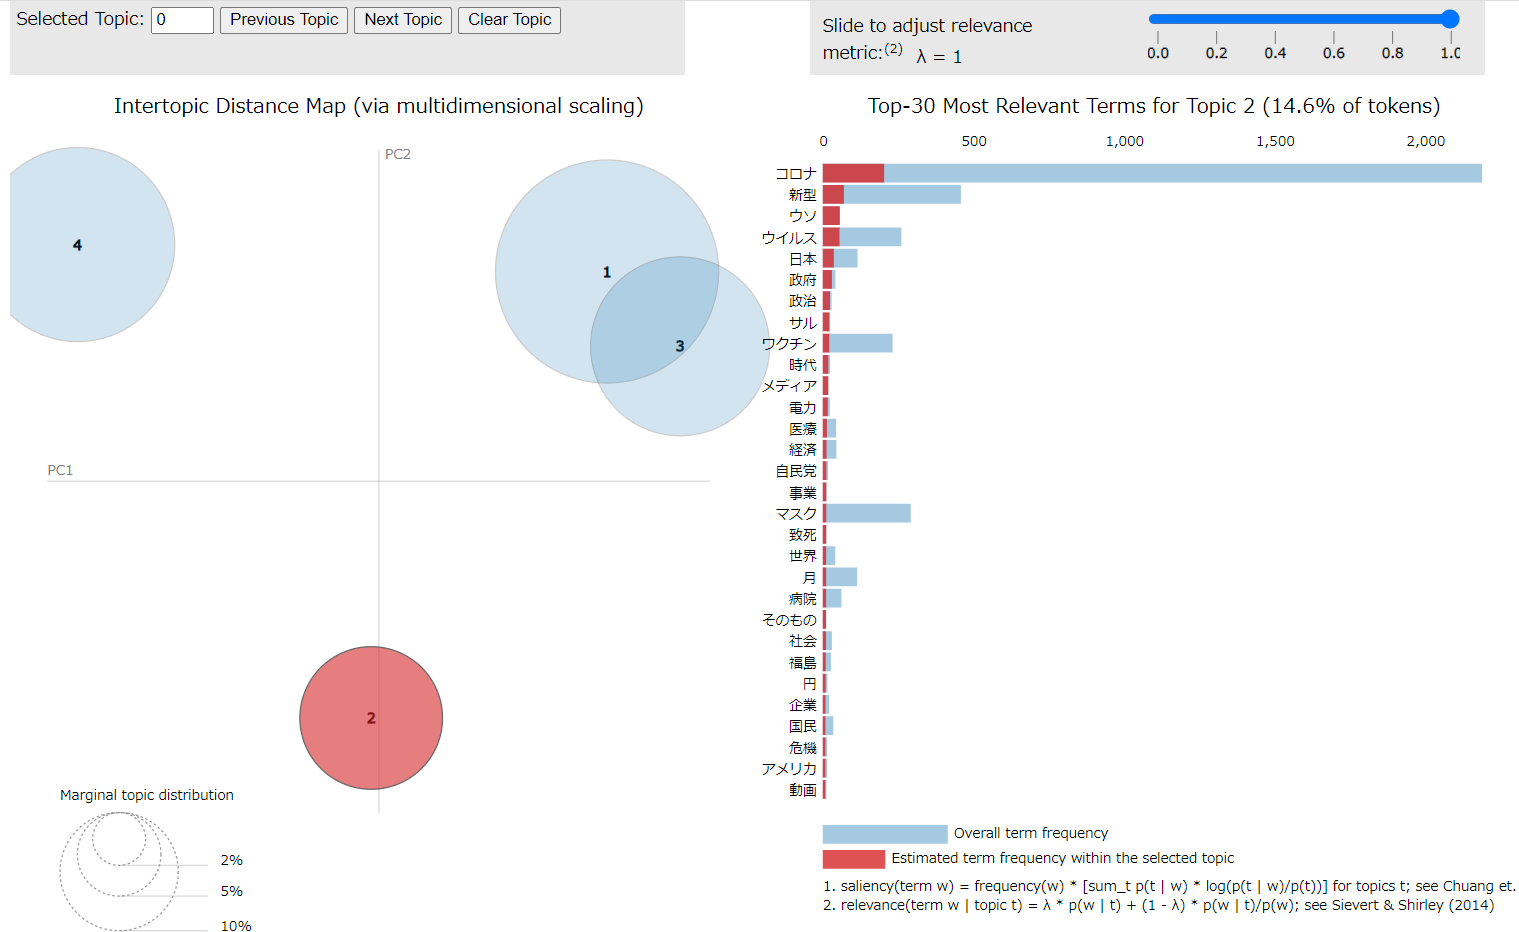
\includegraphics[scale=0.25]{picture4.png}
  \caption{クラス4の単語数}
\end{figure}
また、図5より4のトピックで多い単語は「新型」「ウイルス」「東京」であり、地名や「ニュース」、「新聞」といった単語が4のトピックに多いことがわかる。\\
\begin{figure}[H]
  \centering
  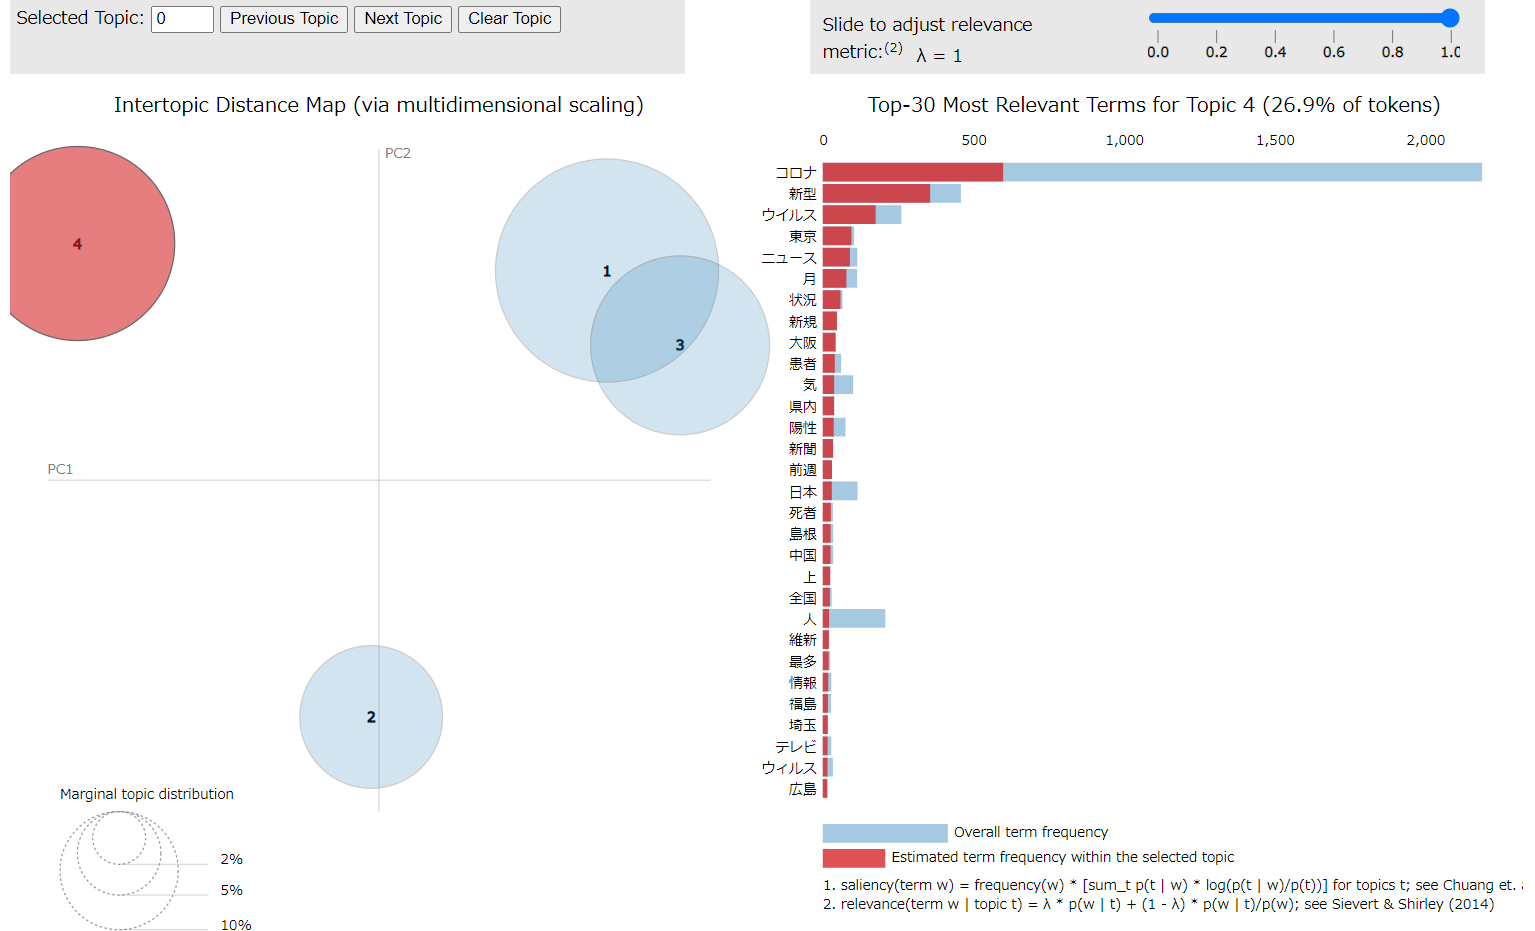
\includegraphics[scale=0.25]{picture5.png}
  \caption{クラス2の単語数}
\end{figure}

\section{考察}
実験結果より、トピック1,3は「コロナ感染症状」、トピック2は「政治」、トピック4は「メディア」の3つのトピックに分けられると考えた。さらに、今回データセットの構築を行う際「コロナ」という単語を含めたツイートを取得していたため、トピックごとに占めるコロナという単語数の割合が多いトピックが今回の実験目的に即していると考える。したがって、コロナによって困っていることのうち、改善する優先度の高いトピックは、コロナ感染症状、ニュース、政治の順であると考える。\\
 しかし、snscrapeを用いて「コロナ」という単語を含めたツイートを取得する際、snscrapeは単語だけでなく、ユーザ名やタグからも取得することに加え、同じtweetにコロナという単語が複数回使われている可能性もある。そのため、一概にコロナという単語数の割合が多ければ優先度の高いトピックとはならない可能性もある。\\
 また、今回の実験は参考資料をもとに行っていたため、LDAのパラメータを理解し、調整するなどを行えていない。今後、より今回の実験に合わせたモデルの構築を行うことができればより良い結果が出るのではないかと考える。また、データの数としてネガティブとして判定されたツイート数は約1万件だった。今回の実験としてこのデータ数が最適なのかということも考えなければならない。

\subsection{追加実験}
(まだ実験していないので書いていません。)

\section{意図していた実験計画との違い}


\section{まとめ}


\begin{thebibliography}{n}
  \bibitem{kanazawa}レポート作成の手引き レポートの基本的形式に関するガイド, \url{https://www.kanazawa-u.ac.jp/wp-content/uploads/2015/01/tebiki2.pdf}, 2020/07/02.
   \bibitem{snscrape}Men of Letters(メン・オブ・レターズ) - 論理的思考/業務改善/プログラミング, \url{https://laboratory.kazuuu.net/using-python-to-scrape-social-networking-sites-using-snscrape/}, 2022/07/02.
    \bibitem{oseti}osetiによる日本語の感情分析, \url{https://note.com/npaka/n/n3c7722d2e4bc}, 2022/07/02.
\bibitem{LDA}Shingoの数学ノート, \url{http://mathshingo.chillout.jp/blog27.html}, 2022/07/05.
      

\end{thebibliography}
\end{document}
